\documentclass[12pt]{article}
\usepackage{amssymb}
\usepackage{geometry}
\usepackage{graphicx}
\usepackage[colorlinks=true, allcolors=blue]{hyperref}
\usepackage{cite}
\usepackage{array}
\usepackage{booktabs}
\usepackage{wrapfig}
\usepackage{amsmath}
\usepackage{lipsum}
\usepackage{caption}
\usepackage{ulem}
\usepackage{xcolor}
\usepackage{tikz}
\usetikzlibrary{arrows.meta, positioning, shapes}

\usepackage{sectsty}
\sectionfont{\color{sectionColor}}       % Color for \section
\subsectionfont{\color{subsectionColor}}


\definecolor{titleColor}{HTML}{800000}        % Maroon
\definecolor{sectionColor}{HTML}{4682B4}      % SteelBlue
\definecolor{textHighlight}{HTML}{DAA520}     % Goldenrod
\definecolor{backgroundColor}{HTML}{F0F8FF}   % AliceBlue
\definecolor{emphasisColor}{HTML}{228B22}     % ForestGreen
\definecolor{subsectionColor}{HTML}{6A5ACD}   % SlateBlue


\title{\textcolor{titleColor}{\textbf{\Huge \textbf{ From Computers to the Heart--Brain System: Signals and Meaning }}}}

\author{B. M. Osman\thanks{Al Nahada University, Cairo \\ \texttt{babikerosman@yahoo.com}}}
\date{\today}
\begin{document}
\maketitle

\section*{Introduction}
At the most fundamental level, all systems of information processing rely on \textit{signals}. 
Computers operate on discrete electrical signals \citep{vonNeumann1945, turing1937}, 
the brain on dynamic electrochemical signals \citep{kandel2000principles, dayan2001theoretical}, 
and the heart--brain system, as conceptualized in the Heart-Based Resonant Consciousness Theory (HBRCT), 
on an integration of electromagnetic and neurochemical signals \citep{mcCraty2003heart, bradley2009electrophysiology}. 
The distinction lies not only in the \textbf{nature of the signals}, but also in how these signals 
are organized to produce \textbf{logic, thought, and meaning}. 
Whereas the computer reduces signals to binary computation, and the brain elevates signals to adaptive thought, 
the heart--brain system transcends both by embedding coherence, emotional tone, and collective resonance. 


\begin{center}
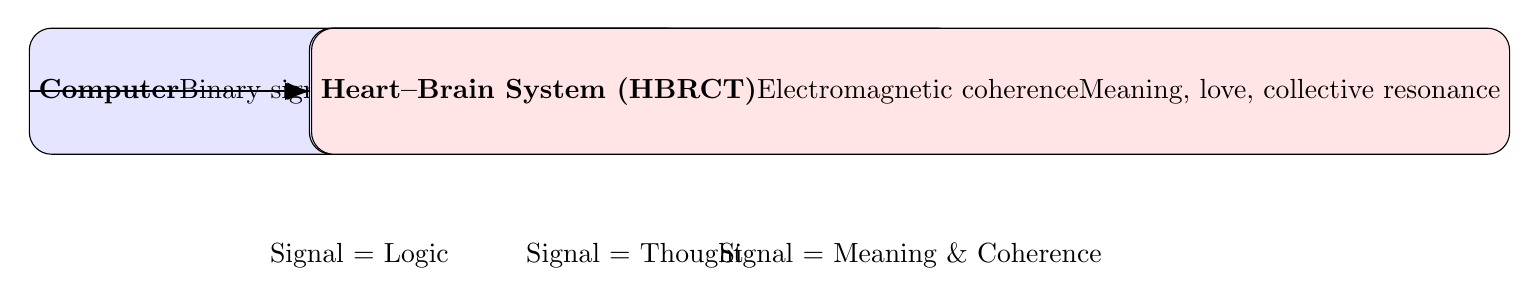
\begin{tikzpicture}[
    node distance=3.5cm,
    box/.style={rectangle, rounded corners=8pt, minimum width=3.8cm, minimum height=1.6cm, text centered, draw=black, fill=blue!10},
    arrow/.style={-{Latex[length=3mm]}, thick}
]

\node[box] (computer) {\textbf{Computer}\\Binary signals (1/0)\\Logic \& computation};
\node[box, right of=computer] (brain) {\textbf{Brain}\\Electrochemical signals\\Thought \& adaptation};
\node[box, right of=brain, fill=red!10] (heartbrain) {\textbf{Heart--Brain System (HBRCT)}\\Electromagnetic coherence\\Meaning, love, collective resonance};

\draw[arrow] (computer) -- (brain);
\draw[arrow] (brain) -- (heartbrain);

\node[below=1cm of computer] {Signal = Logic};
\node[below=1cm of brain] {Signal = Thought};
\node[below=1cm of heartbrain] {Signal = Meaning \& Coherence};

\end{tikzpicture}
\end{center}

\section*{Tabular Comparison}

\begin{tabular}{>{\raggedright\arraybackslash}p{3cm} 
                >{\raggedright\arraybackslash}p{4cm} 
                >{\raggedright\arraybackslash}p{4cm} 
                >{\raggedright\arraybackslash}p{4cm}}
\toprule
\textbf{Aspect} & \textbf{Computer} & \textbf{Brain} & \textbf{Heart--Brain System (HBRCT)} \\
\midrule
Nature of Signals 
& Electrical (binary on/off, 1s and 0s) 
& Electrochemical (neural firing, continuous and adaptive) 
& Electromagnetic and neurochemical (heart rhythms generating coherence) \\
\midrule
Processing Units 
& Transistors and logic gates 
& Neurons and synapses 
& Heart field + brain networks in resonance \\
\midrule
Information Handling 
& Fixed rules, programmed logic 
& Learning and neuroplasticity 
& Meaning, coherence, and resonance (integration of emotion and intuition) \\
\midrule
Source of Purpose 
& External programmer 
& Experience and memory 
& Intrinsic resonance, love, and collective consciousness \\
\midrule
Output 
& Logical results, computations 
& Thoughts, perceptions, adaptive behavior 
& Coherence, intuitive insight, collective field of consciousness \\
\bottomrule
\end{tabular}

\section*{Visual Representation}

\begin{center}
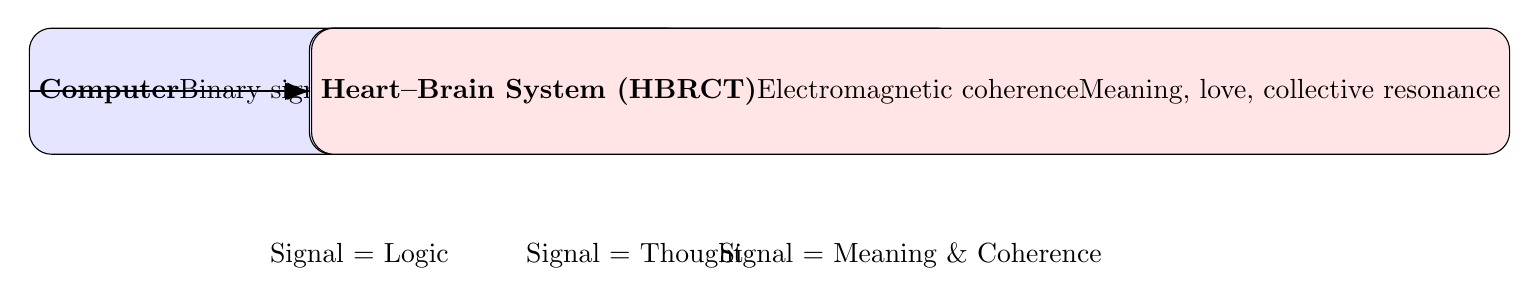
\begin{tikzpicture}[
    node distance=3.5cm,
    box/.style={rectangle, rounded corners=8pt, minimum width=3.8cm, minimum height=1.6cm, text centered, draw=black, fill=blue!10},
    arrow/.style={-{Latex[length=3mm]}, thick}
]

% Nodes
\node[box] (computer) {\textbf{Computer}\\Binary signals (1/0)\\Logic \& computation};
\node[box, right of=computer] (brain) {\textbf{Brain}\\Electrochemical signals\\Thought \& adaptation};
\node[box, right of=brain, fill=red!10] (heartbrain) {\textbf{Heart--Brain System (HBRCT)}\\Electromagnetic coherence\\Meaning, love, collective resonance};

% Arrows
\draw[arrow] (computer) -- (brain);
\draw[arrow] (brain) -- (heartbrain);

% Labels
\node[below=1cm of computer] (lab1) {Signal = Logic};
\node[below=1cm of brain] (lab2) {Signal = Thought};
\node[below=1cm of heartbrain] (lab3) {Signal = Meaning \& Coherence};

\end{tikzpicture}
\end{center}


\section*{Synthesis}
This progression from \textbf{logic (computer)} to \textbf{thought (brain)} to \textbf{meaning and coherence (heart--brain)} 
highlights a spectrum of signal organization. 
The computer demonstrates the foundation of physical signal dependency, 
the brain introduces adaptability and cognition, 
and the heart--brain system integrates a higher dimension of coherence, 
linking individual consciousness to a collective field. 

In this way, HBRCT proposes that the heart is not merely a physiological pump, 
but a resonant integrator of signals, encoding meaning, intuition, and love into the dynamics of consciousness 
\citep{mcCraty2015science, childre2016heartintelligence}.


\section*{Conclusion}
The transition from computer logic to brain thought to heart coherence represents an evolutionary 
deepening of signal processing: from raw computation, to adaptive cognition, to the emergence of 
meaning and resonance. This layered view situates HBRCT as a new framework for unifying 
biological, computational, and conscious processes.


\nocite{*}
\bibliographystyle{plain}
\bibliography{ref}
\end{document}
\bibliographystyle{apalike}

